\section{Experiments and Results}

\begin{frame}
\frametitle{Robot Planner 1: Simple MoveIt planning}
\end{frame}

\begin{frame}
\frametitle{Robot Planner 2: Simulation layout and reachability experiments}
\end{frame}

\begin{frame}
\frametitle{Robot Planner 3b: Line segment trajectories in task space}
\end{frame}

\begin{frame}
\frametitle{Robot Planner 3a: Circular and Circular arc trajectories in task space}
\end{frame}

\begin{frame}
\frametitle{Robot Planner 3h: Helical trajectories in task space}
\end{frame}

\begin{frame}
\frametitle{Robot Planner 4: Simple cube pick-and-place experiment}
\end{frame}

\begin{frame}
\frametitle{Robot Planner 5: Visual servoing}
\begin{center}
\begin{figure}[!htb]
\centering
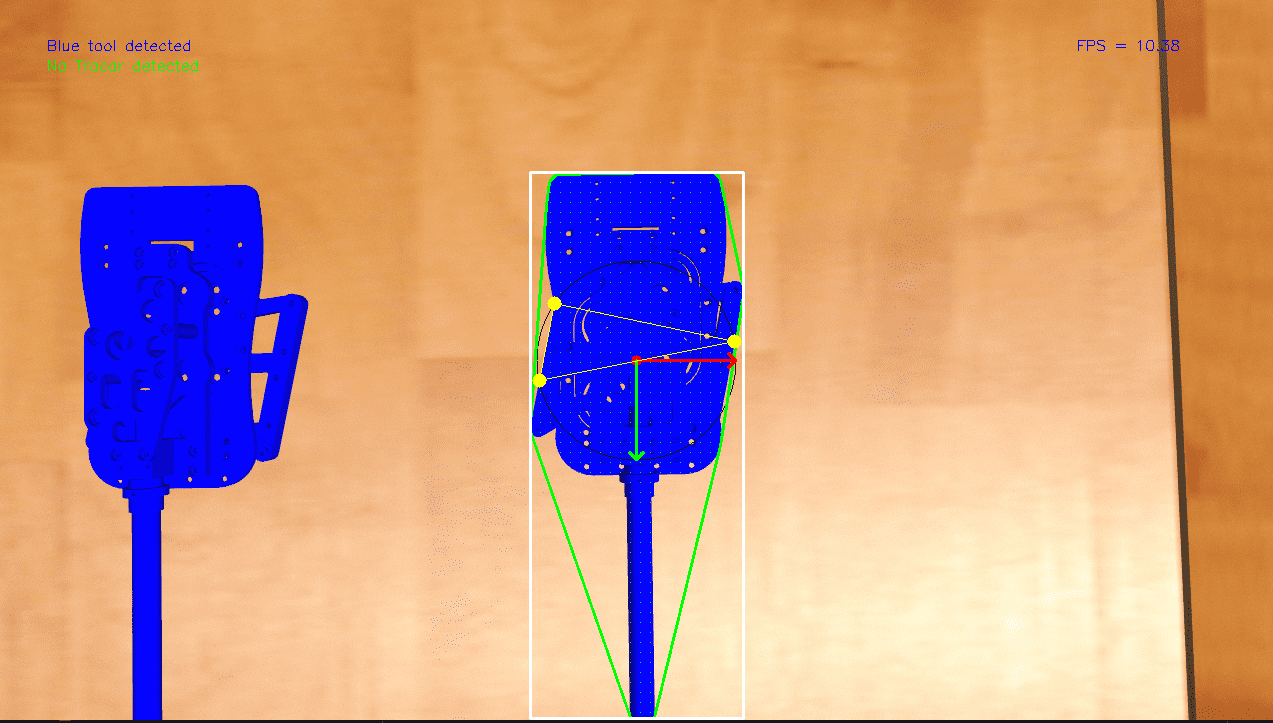
\includegraphics[width=0.6\textwidth]{../images/grasp-points-triangle.png}\\
\caption{Image based visual servoing and calculation of grasp points. The yellow points are the grasp points and the thin black circumscribed circle is the growing circle that was used to calculate them.}
\end{figure}
\end{center}
\end{frame}

\begin{frame}
\frametitle{Robot Planner 5: Visual servoing}
\begin{center}
\begin{figure}[!htb]
\centering
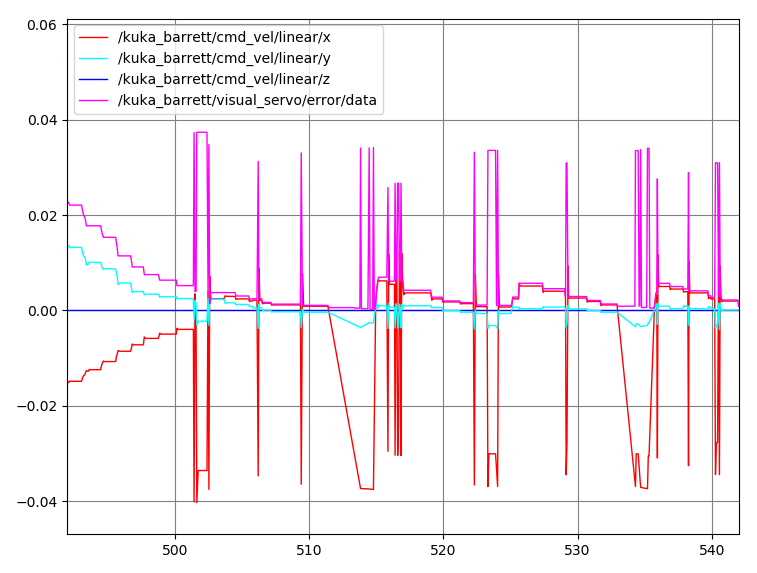
\includegraphics[width=0.45\textwidth]{../images/robot_planner5/visual_servo_controller3.png}
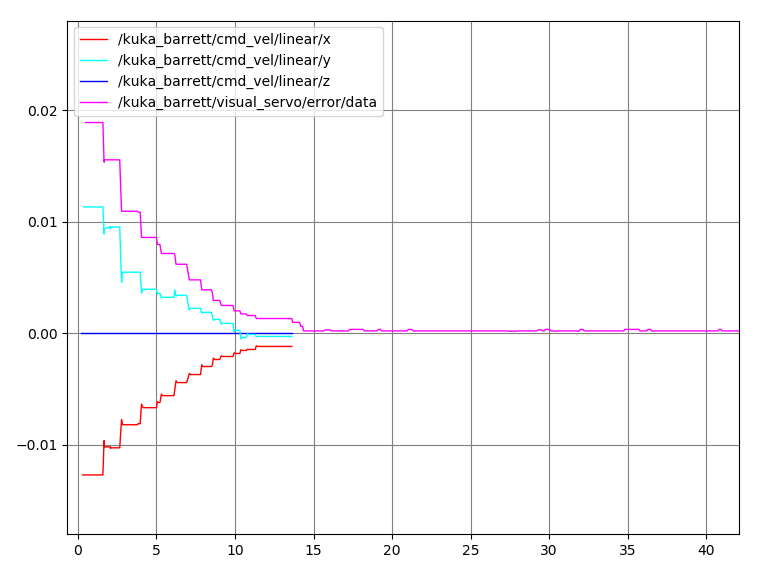
\includegraphics[width=0.45\textwidth]{../images/robot_planner5/visual_servo_controller4.png}\\
\caption{Visual servo controller error diagrams. On the left image in the error graphs appear some spikes. These spikes occur from the sudden temporary detection 
of a nearby surgical tool. On the right image, these spikes are filtered out, and only the error graphs of the visual servoing of one tool are shown. The  
controller parameters are $K_p = 0.9, K_d = 0.2$}
\end{figure}
\end{center}
\end{frame}

\begin{frame}
\frametitle{Robot Planner 6: RCM alignment error in insertion and retraction}
\end{frame}

\begin{frame}
\frametitle{Robot Planner 7: State machine - End-to-end simulation}

\begin{columns}

\column{0.6\textwidth}
\begin{center}
\begin{figure}[!htb]
\centering
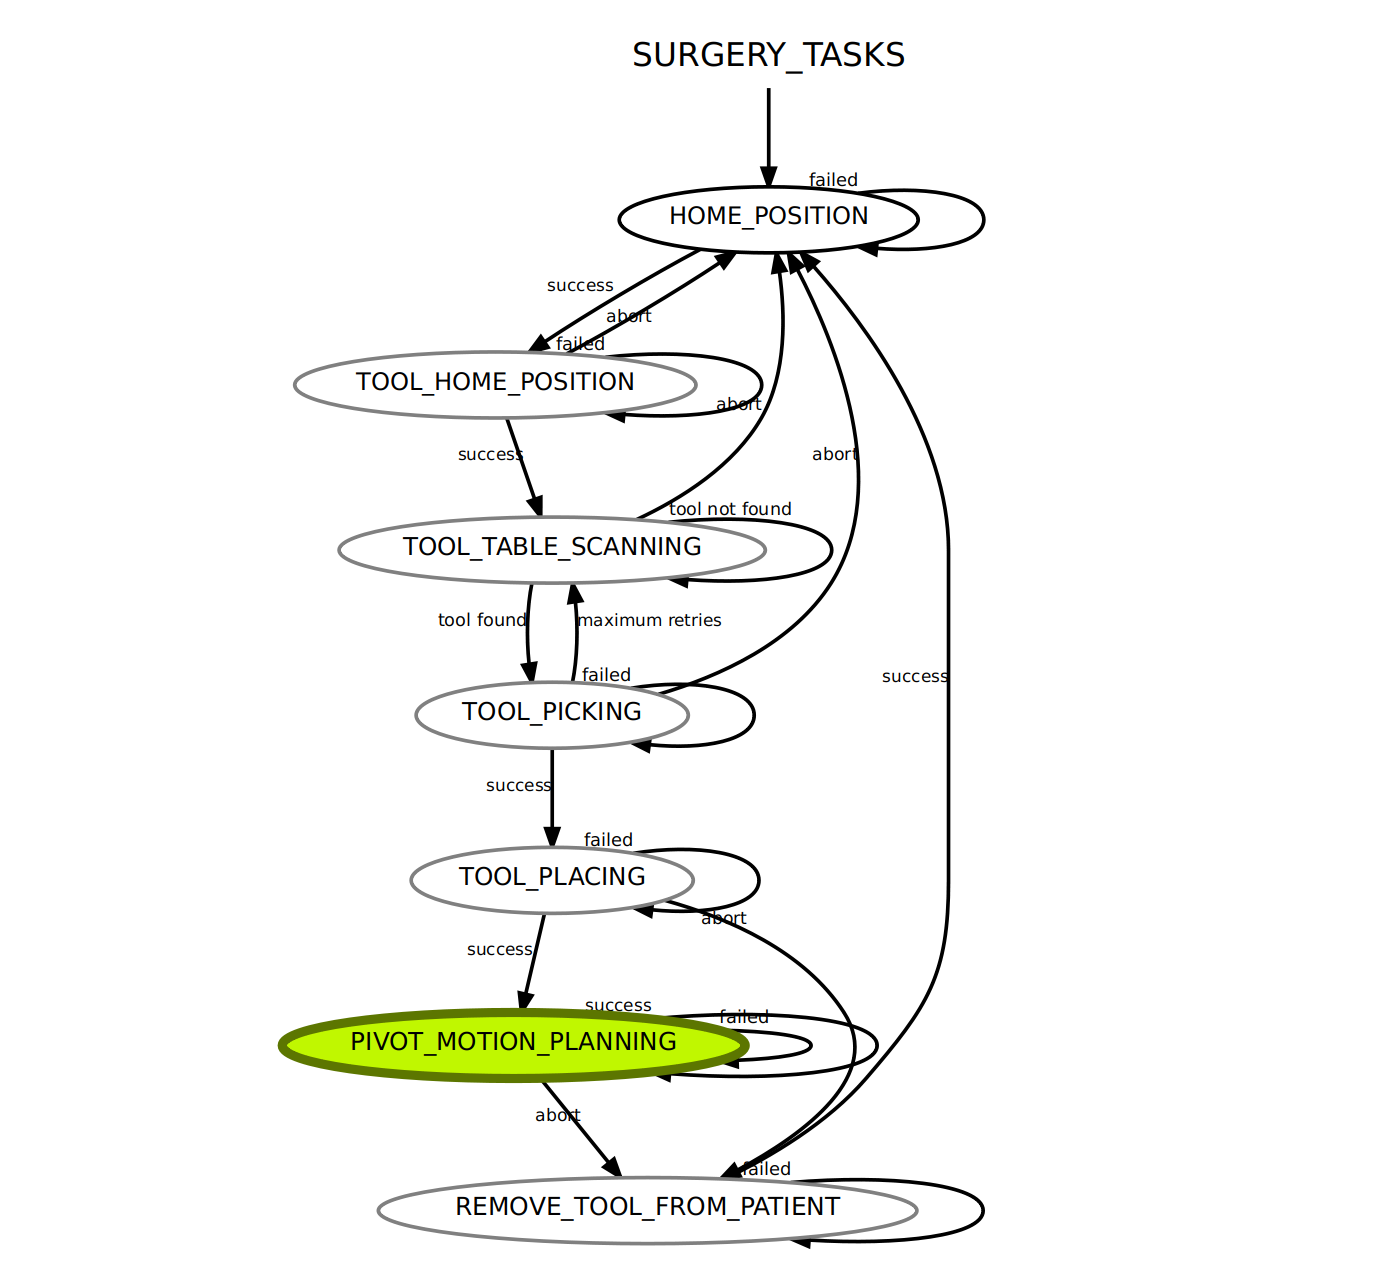
\includegraphics[width=\textwidth]{../images/state-machine-all-tasks.png}
\label{smack-state-machine}
\end{figure}
\end{center}

\column{0.3\textwidth}
Run all the stages of this thesis together (integration testing) using a state machine.
\end{columns}
\end{frame}


\begin{frame}
\frametitle{Demo}
\begin{center}
\begin{figure}[!htb]
\centering
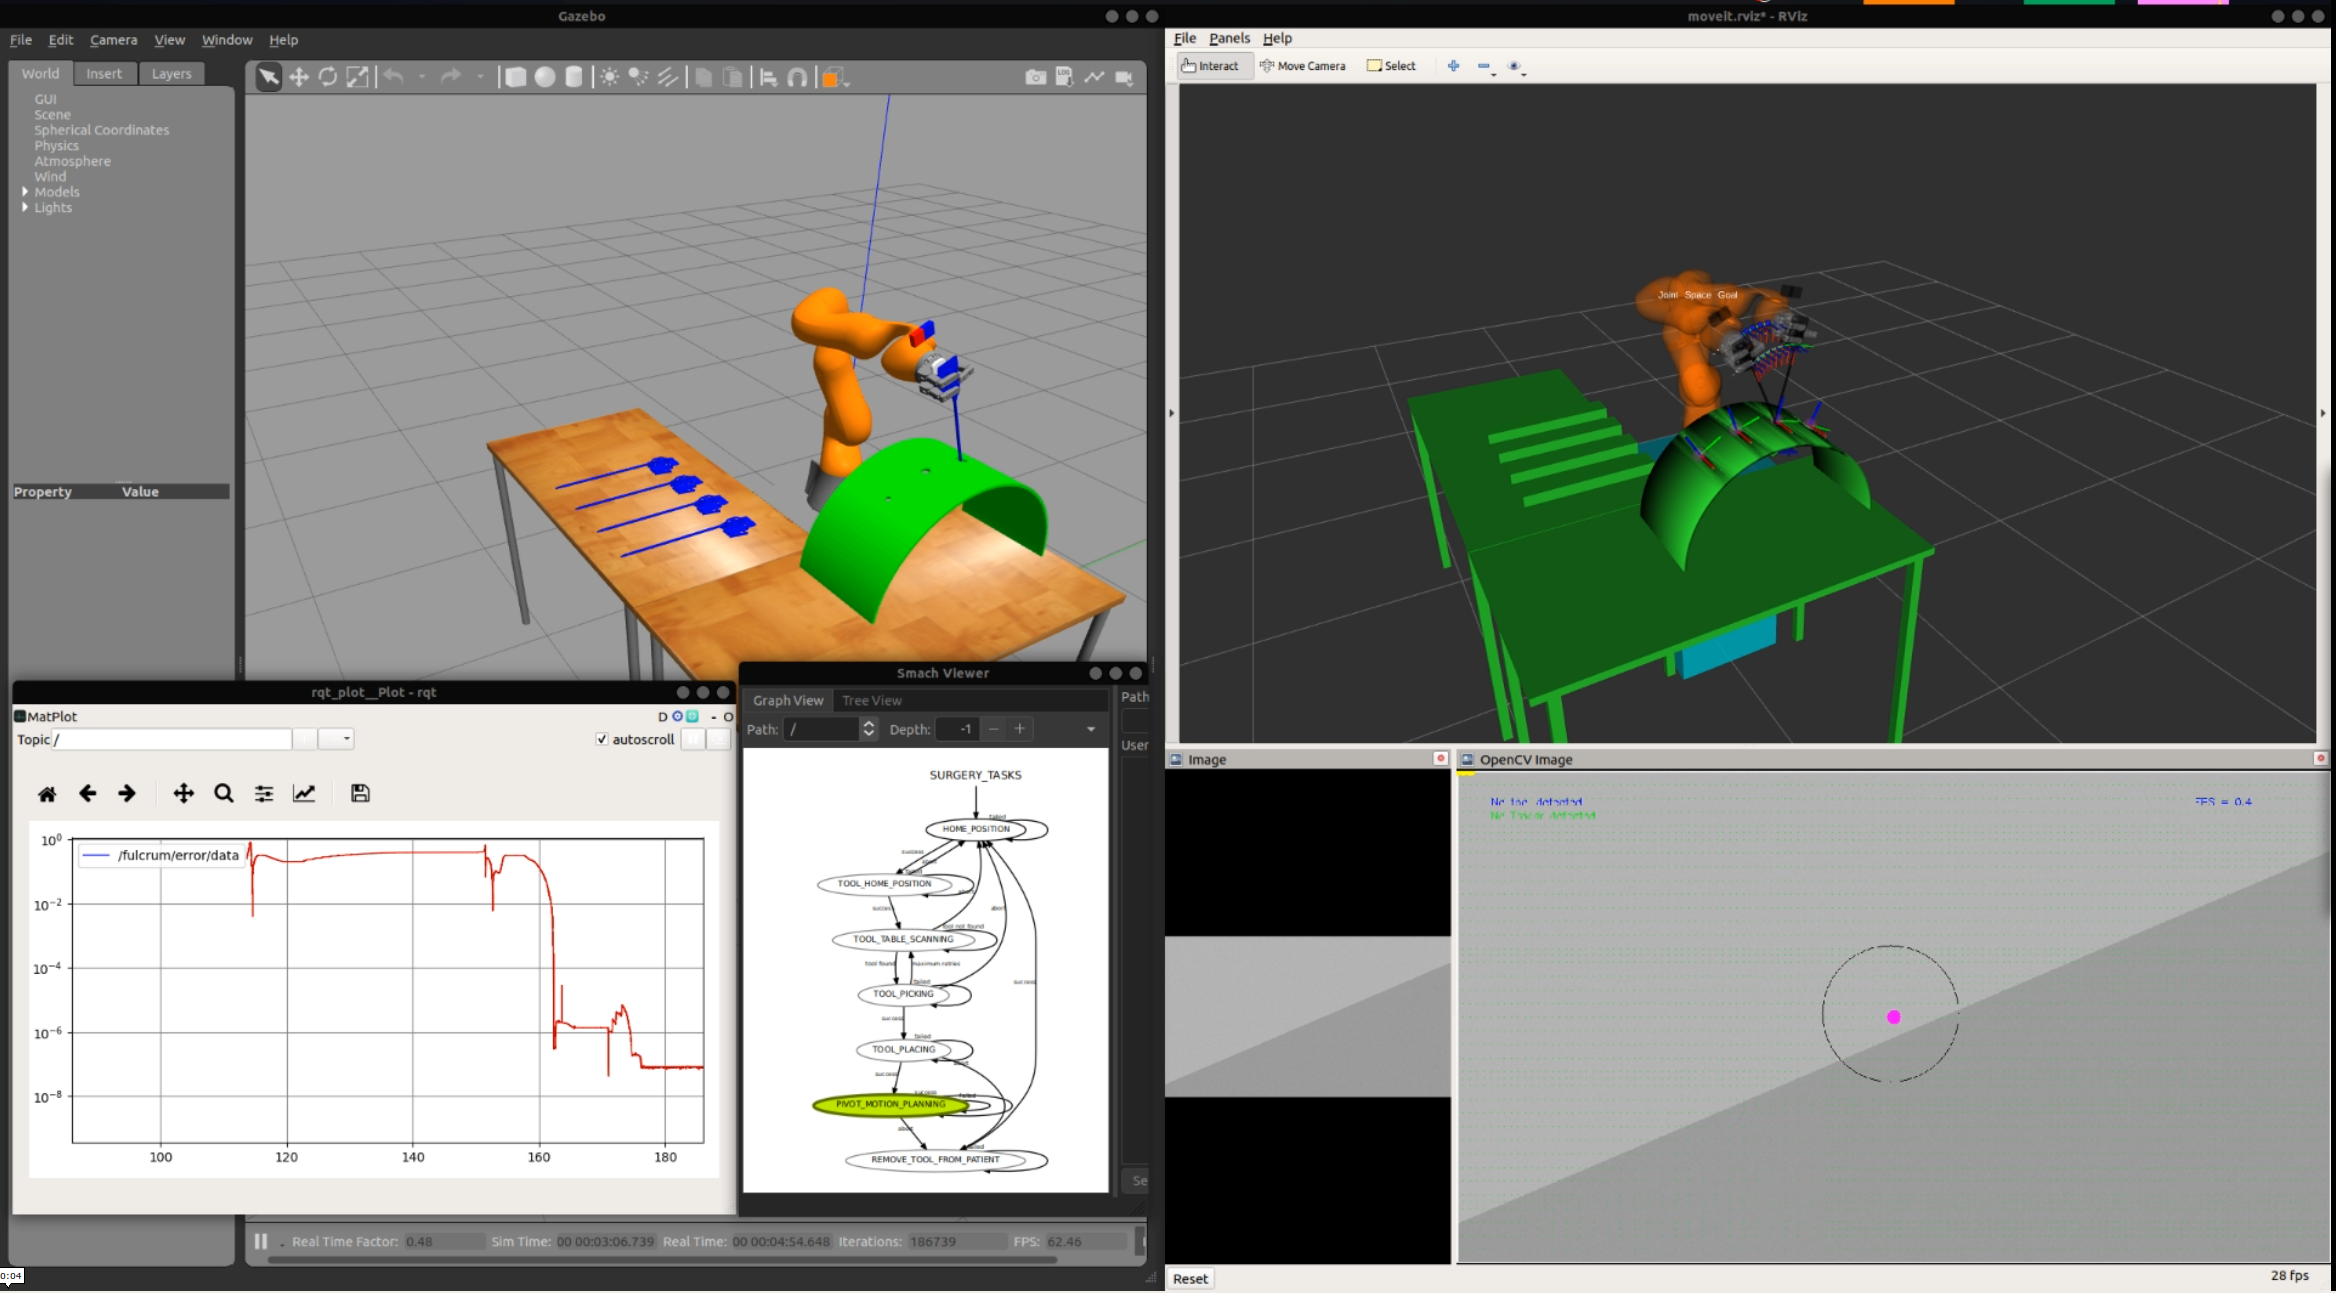
\includegraphics[width=\textwidth]{../images/demo.png}\\
\end{figure}
\url{https://youtu.be/lfV1vdHf7bk}
\end{center}
\end{frame}
